\chapter*{Dodatak: Prikaz aktivnosti grupe}
		\addcontentsline{toc}{chapter}{Dodatak: Prikaz aktivnosti grupe}
		
		\section*{Dnevnik sastajanja}
		
		\begin{packed_enum}
			\item  sastanak
			
			\item[] \begin{packed_item}
				\item Datum: 23. listopada 2023.
				\item Prisustvovali: Hrvoje Cerin, Leon Tišljarić, Matko Ljepović,  Šimun Banović
				\item Teme sastanka:
				\begin{packed_item}
					\item  Raspodjela poslova
					\item  Upoznavanje članova tima
					\item  Nazočnost na CROZ predavanju
				\end{packed_item}
			\end{packed_item}
			
			\item  sastanak
			\item[] \begin{packed_item}
				\item Datum: 9. studenoga 2023.
				\item Prisustvovali: Hrvoje Cerin, Leon Tišljarić, Matko Ljepović,  Dan Široki
				\item Teme sastanka:
				\begin{packed_item}
					\item  Dogovor vezani uz implementaciju stavki
					\item  Proučavanje primjera dokumentacije
					\item  Nazočnost na CROZ predavanju
				\end{packed_item}
			\end{packed_item}
			
			%
			
		\end{packed_enum}
		
		\eject
		\section*{Tablica aktivnosti}
		
			\textbf{\textit{Kontinuirano osvježavanje}}\\
			
			 \textit{Napomena: Doprinose u aktivnostima treba navesti u satima po članovima grupe po aktivnosti.}

			\begin{longtblr}[
					label=none,
				]{
					vlines,hlines,
					width = \textwidth,
					colspec={X[7, l]X[1, c]X[1, c]X[1, c]X[1, c]X[1, c]X[1, c]X[1, c]}, 
					vline{1} = {1}{text=\clap{}},
					hline{1} = {1}{text=\clap{}},
					rowhead = 1,
				} 
			
				\SetCell[c=1]{c}{} & \SetCell[c=1]{c}{\rotatebox{90}{\textbf{Hrvoje Cerin}}} & \SetCell[c=1]{c}{\rotatebox{90}{\textbf{Leon Tišljarić }}} &	\SetCell[c=1]{c}{\rotatebox{90}{\textbf{Dan Široki }}} & \SetCell[c=1]{c}{\rotatebox{90}{\textbf{Matko Ljepović }}} &	\SetCell[c=1]{c}{\rotatebox{90}{\textbf{Šimun Banović }}} & \SetCell[c=1]{c}{\rotatebox{90}{\textbf{-}}} &	\SetCell[c=1]{c}{\rotatebox{90}{\textbf{-}}} \\  
				Upravljanje projektom 		&x  &  &  &  &  &  & \\ 
				Opis projektnog zadatka 	&  &x  &  &  &  &  & \\ 
				
				Funkcionalni zahtjevi       &x  &x  &x  &x  &x  &  &  \\ 
				Opis pojedinih obrazaca 	&  &  &  &  &  &  &  \\ 
				Dijagram obrazaca 			&  &  &  &  &  &  &  \\ 
				Sekvencijski dijagrami 		&  &  &  &  &  &  &  \\ 
				Opis ostalih zahtjeva 		&  &  &  &  &  &  &  \\ 

				Arhitektura i dizajn sustava	 &x  &x  &  &  &x  &  &  \\ 
				Baza podataka				&x  &  &  &x  &x  &  &   \\ 
				Dijagram razreda 			&  &  &  &  &x  &  &   \\ 
				Dijagram stanja				&  &  &x  &  &  &  &  \\ 
				Dijagram aktivnosti 		&  &  &x  &  &  &  &  \\ 
				Dijagram komponenti			&  &  &  &  &  &  &  \\ 
				Korištene tehnologije i alati 		&  &  &  &  &  &  &  \\ 
				Ispitivanje programskog rješenja 	&  &  &  &  &  &  &  \\ 
				Dijagram razmještaja			&  &  &x  &  &  &  &  \\ 
				Upute za puštanje u pogon 		&  &  &  &  &  &  &  \\  
				Dnevnik sastajanja 			&  &  &  &  &  &  &  \\ 
				Zaključak i budući rad 		&  &  &  &  &  &  &  \\  
				Popis literature 			&  &  &  &  &  &  &  \\  
				&  &  &  &  &  &  &  \\ \hline 
				\textit{Dodatne stavke} 			&  &  &  &  &  &  &  \\ 
				\textit{Front end}		&  &x  &x  &  &  &  &  \\
				\textit{Izrada početne stranice} 				&  &x  &x  &  &  &  &  \\  
				\textit{Izrada side bar-a} 				&  &x  &  &  &  &  &  \\  
				\textit{Izrada stranice za login i registraciju} 				&  &x  &  &  &  &  &  \\  
				\textit{Back end} 							&x  &  &  &x  &x  &  &  \\  
				\textit{Izrada baze podataka} 		 			&x  &  &  &x  &x  &  & \\  
				\textit{Spajanje s bazom podataka} 							&x  &x  &  &x  &x  &  &  \\ 
				\textit{Deployment}		&x	&	&	&	&	&	&\\
				 							&  &  &  &  &  &  &\\ 
			\end{longtblr}
					
					
		\eject
		\section*{Dijagrami pregleda promjena}
			\begin{figure}
				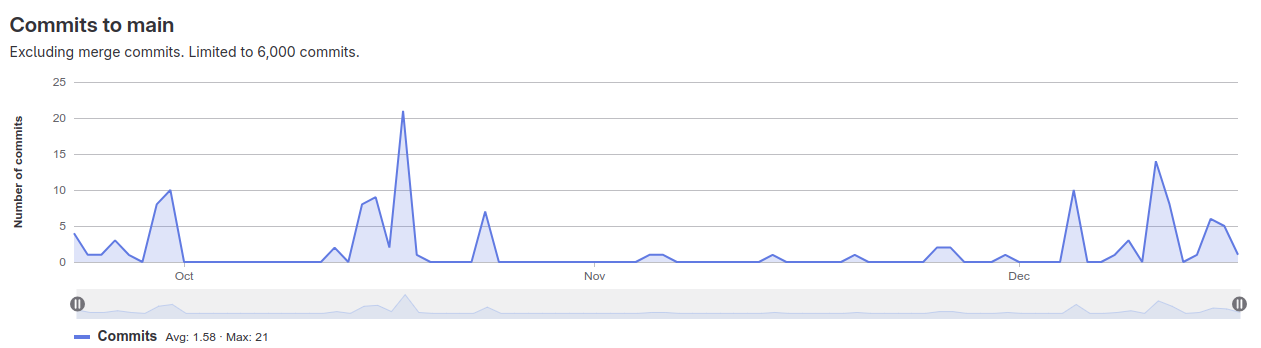
\includegraphics[width=15cm]{dijagrami/dijagram_pregleda_promjena.png}
			\end{figure}
			\begin{figure}
				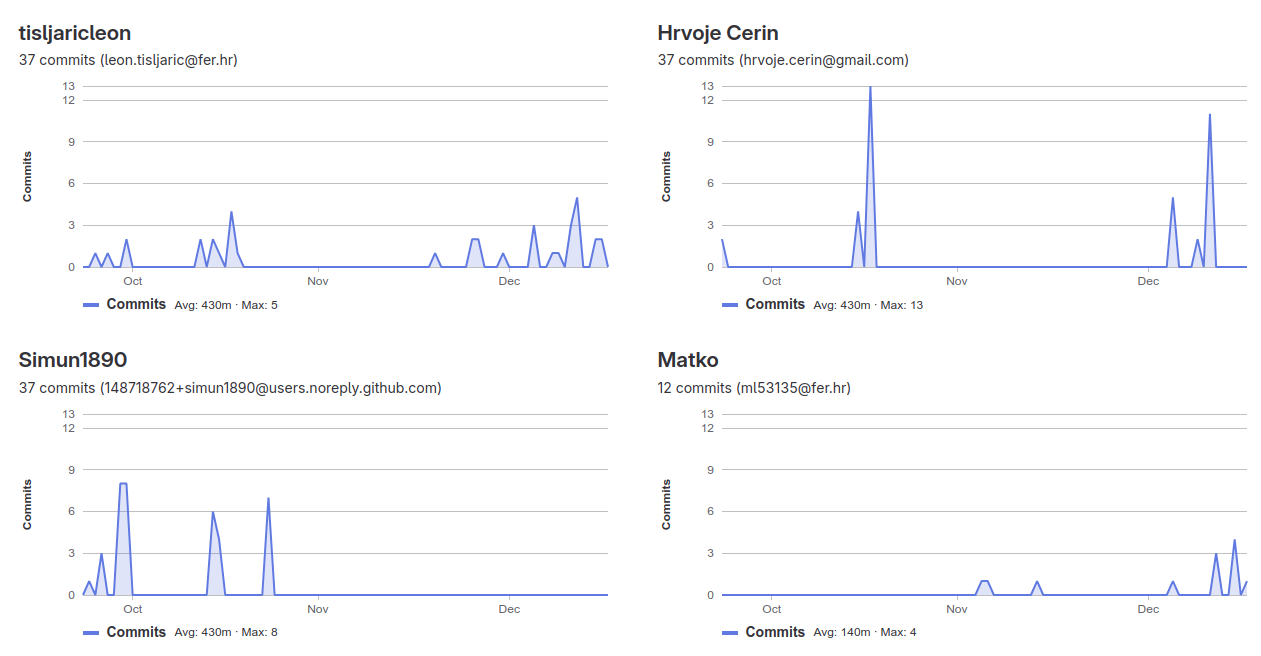
\includegraphics[width=15cm]{dijagrami/dijagram_pregleda_promjena2.png}
			\end{figure}
			\begin{figure}
				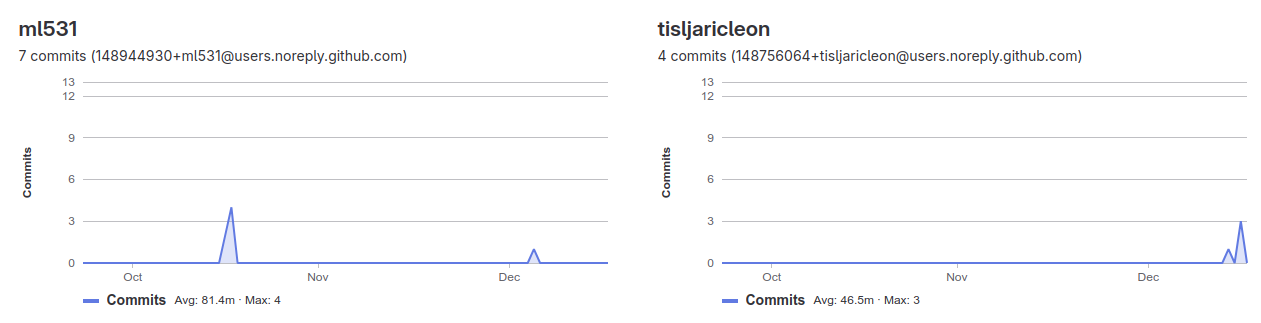
\includegraphics[width=15cm]{dijagrami/dijagram_pregleda_promjena3.png}
			\end{figure}
			\textit{Prenijeti dijagram pregleda promjena nad datotekama projekta. Potrebno je na kraju projekta generirane grafove s gitlaba prenijeti u ovo poglavlje dokumentacije. Dijagrami za vlastiti projekt se mogu preuzeti s gitlab.com stranice, u izborniku Repository, pritiskom na stavku Contributors.}
		\eject
		
	
